\chapter{Vorstellung von Apache Spark}
Aus Sicht eines Nutzers ist Apache Spark eine API zum Zugriff auf Daten und deren Verarbeitung.\\

Diese API (wahlweise für die Programmiersprachen Scala, Java und Python verfügbar), kann im einfachsten Fall über eine eigene Spark Konsole mit \gls{repl}\footcite{Hail} verwendet werden.\\
Die Zählung von Wortvorkommen in einem Text - das "`Hello World"' der Big Data Szene - lässt sich dort mit zwei Befehlen realisieren (Listing 2.1).\\

\begin{lstlisting}[caption=Word Count in der Spark Konsole]
my_dollar ./spark-shell
[...]
     / __/__  ___ _____/ /__
    _\ \/ _ \/ _ `/ __/  '_/
   /___/ .__/\_,_/_/ /_/\_\   version 1.3.0
      /_/
Using Scala version 2.10.4 (OpenJDK 64-Bit Server VM, Java 1.7.0_75)
Type in expressions to have them evaluated.
[...]
scala> val text = sc.textFile("../Heinrich Heine - Der Ex-Lebendige")
[...]
scala> :paste
text.flatMap(line => line.split(" "))
.map(word => (word, 1))
.reduceByKey(_ + _)
.collect()
[...]
res0: Array[(String, Int)] = Array((Tyrann,,1), (im,2), (Doch,1) ...)

\end{lstlisting}


Aus Sicht eines Administrators oder Softwarearchitekten ist Apache Spark eine Applikation auf einem \gls{cluster}, die sich in der Anwendungsschicht befindet und charakteristische Anforderungen insbesondere an Lokalität des Storages und die Netzwerkperformance stellt.\\

Was das konkret bedeutet, welche Mechanismen und Konzepte dahinterstehen und in welchem Ökosystem von Anwendungen sich Apache Spark bewegt wird in den folgenden Abschnitten dieses Kapitels beleuchtet.

\section{Überblick}
Im Allgemeinen Fall läuft eine Spark-Anwendung auf drei Arten von Rechnern (s. Abb. \ref{figure:sparkdeployment}):

\begin{enumerate}
	\item \textbf{Clientknoten}\\
	Auf Nutzerseite greift die Anwendung auf die API eines lokalen Spark-Kontextes zu, der die Kontaktdaten eines Clustermanagers sowie verschiedene Konfigurationseinstellungen enthält. 
	
	\item \textbf{\gls{master}knoten}\\
	Der \gls{master}knoten betreibt den \textit{Clustermanager} läuft auf einem entfernten Rechner und ist der Einstiegspunkt in den \gls{cluster}. Hier werden Aufträge des Anwenders an die Arbeitsknoten verteilt und Ergebnisse eingesammelt und zurückgereicht.
	
	\item \textbf{\gls{worker}knoten}\\
	Die \gls{worker}knoten beherbergen die Spark \textit{Executors} und sind die ausführenden Elemente der Aktionen und Transformationen. Die \textit{Executors} können untereinander Zwischenergebnisse austauschen und melden ihre Ressourcenverfügbarkeit an den \textit{Clustermanager}.
\end{enumerate}

\begin{figure}[ht!]
	\centering
  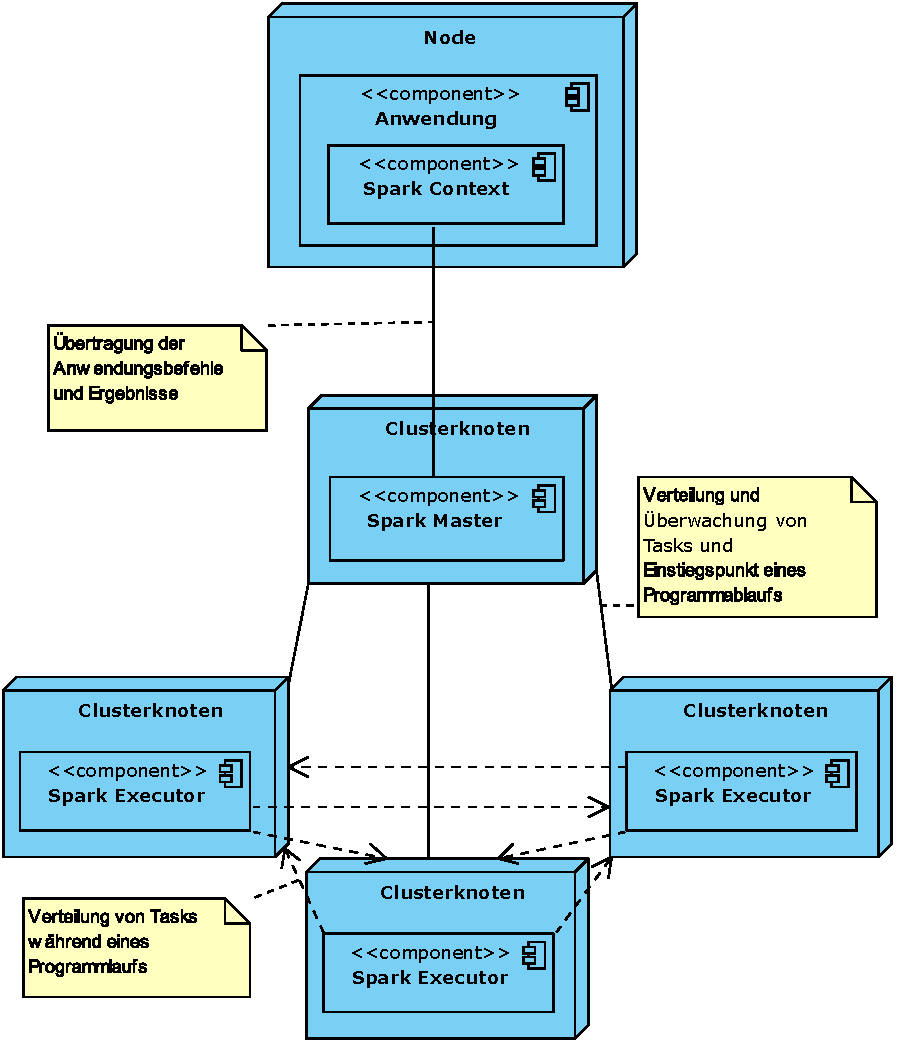
\includegraphics[pdf,scale=0.7]{sparkdeployment2}
	\caption{Verteilungsdiagramm einer typischen Sparkinstallation}
	\label{figure:sparkdeployment}
\end{figure}

Um die Architektur und Optimierungskonzepte eines verteilten Systems bewerten zu können ist es offensichtlich wichtig, welche Eigenschaften der unterliegenden Hardware angenommen werden.

Weil Spark explizit für den Betrieb innerhalb eines Hadoop/YARN \textcolor{red}{[VERWEIS auf Abschnitt Scheduling]} geeignet ist und YARN wiederum für den Betrieb auf einem \gls{cluster} auf Mittelklasse-Mehrzweckmaschinen (Commodity Hardware) optimiert ist\footcite{Mer14}, kann für Spark von einer vergleichbaren Hardwarekonfiguration ausgegangen werden.\\

Der Vergleich von drei aktuellen Rack Servern der 2000-Euro-Klasse (in der Grundausstattung) - hier als Mittelklasse-Geräte bezeichnet - liefert die folgenden Verhältnisse der wesentlichen Schnittstellen zueinander (Siehe Anhang~\ref{subsec:commodity_servers}).

\begin{table}[ht]
	\centering % used for centering table
	\begin{tabular}{c c c} % centered columns (4 columns)	
		\hline\hline %inserts double horizontal lines
		Netzwerk & Festspeicher & Arbeitsspeicher\\ [0.5ex] % inserts table
		%heading
		\hline % inserts single horizontal line
		0,125 GB/s & 1 GB/s & 17 GB/s \\ % inserting body of the table
		\hline %inserts single line
	\end{tabular}
	\caption{Theoretische Spitzenleistungen bei Mittelklasse-Servern} % title of Table
	\label{table:vgldurchsatz} % is used to refer this table in the text
\end{table}

Auf eine detaillierte Analyse des Zugriffsverhaltens wird im Rahmen dieser Arbeit verzichtet. Bei den folgenden Bewertungen der Kernkonzepte ist es wichtig sich die aus Tabelle \ref{table:vgldurchsatz} abgeleiteten Größenordnungen des Durchsatzes (\textit{D}) der verschiedenen Datenkanäle zu vergegenwärtigen:

\begin{equation*}
	D_{Netzwerk} < D_{Festspeicher} < D_{Arbeitsspeicher}
\end{equation*}

Für eine effiziente Verarbeitung von Daten ist es - ganz allgemein - also wünschenswert den größten Anteil des Datentransfers im Arbeitsspeicher zu haben, einen kleineren Anteil auf der Festplatte und einen noch kleineren Anteil auf Netzwerkverbindungen.\\

Es ist das oberste Ziel der folgenden Kernkonzepte von Apache Spark unter diesen Bedingungen die effiziente Verarbeitung \textit{großer Datenmengen}\footcite{Sam14} zu gewährleisten.\\

\section{Kernkonzepte}
Die universelle Einheit mit der ein Datenelement auf Spark repräsentiert wird ist ein sogenanntes \gls{rdd}\footcite{Mat12}.
Die gesamte operative Kern-API dreht sich um die Steuerung dieser Datenelemente. Insbesondere sind auch die in den Standardbibliotheken verfügbaren "`höheren"' APIs auf diesen \glspl{rdd} implementiert.

\glspl{rdd} sind damit die wichtigste Abstraktion des Applikationskerns.

In erster Näherung können \glspl{rdd} als eine Variante von \gls{dsm}\footcite{Nitzberg:1991:DSM:112827.112855} \cite{Mat12} verstanden werden, haben allerdings sehr charakteristische Einschränkungen und Erweiterungen, die im Folgenden erläutert werden.\\



\subsection{Nutzung von Arbeitsspeicher}

\subsection{Nutzung von persistentem Speicher}
\subsection{Nutzung von CPUs}
\subsection{Scheduling/Shuffling}
\subsection{Kern-API}
\paragraph{Transformationen}
\paragraph{Aktionen}

\section{Standardbibliotheken}
\textcolor{gray}{--- Warum ist Spark so einfach (und wo vielleicht nicht)? ---}\\
Die vier Standardbibliotheken erweitern die Kern-API für bestimmte, häufig genutzte Aufgaben aus Bereichen der Datenanalyse.\\

Die bedienten Bereiche sind
\begin{itemize}
	\item Deklaratives Abfragen auf strukturierten Datensätzen (\textit{Spark SQL})
	\item Maschinenlernverfahren (\textit{MLlib})
	\item Echtzeitbehandlung von eingehenden Daten (\textit{Streaming})
	\item Operationen auf Graph-Strukturen (\textit{GraphX})
\end{itemize}

\subsection{Dataframes/Spark SQL}
\subsection{MLlib}
\subsection{Streaming}
\subsection{GraphX}

\section{Betrieb und Security}

\section{Spark im Kontext von Parallelisierungspattern}
\textcolor{gray}{--- Buch: Algorithms and Parallel Computing ---}\\

\section{Entwicklergemeinschaft}
\textcolor{gray}{--- Herkunft, Apache Foundation, Entwicklungsphilosophien, Anzahl Entwickler, ... ---}\\

\section{Verwandte Produkte}
\textcolor{gray}{--- Ergänzende oder konkurrierende Produkte ---}\\
\subsection{YARN}
\subsection{Mesos}
\subsection{Flink}
\subsection{MPI}
\subsection{Kafka}
\subsection{HBase}
\subsection{Lustre}
